\chap{Changer les couleurs}

\sect{Colorer Thymio}

\begin{bclogo}[couleur = pink!30, arrondi = 0.1, logo = \bccrayon, ombre = true]{Challenge!}Écrivez un programme en utilisant VPL qui affiche deux couleurs différentes sur le dessus de Thymio lorsque le bouton avant ou arrière est pressé et deux autres couleurs sous Thymio lorsque le bouton gauche ou droite est pressé.
\end{bclogo}

{\raggedleft \hfill Programme: \bu{colors.aesl}}

Nous avons besoin de quatre paires d'événement-action puisqu'il y a quatre conditions. Les quatre événements sont la pression des quatre boutons en forme de triangle de Thymio. Chacun de ces événements doit être associé avec une action de couleur. Vous verrez qu'il y a une différence entre l'icône \blk{action-colors-up-white} et l'icône \blk{action-colors-down-white}. La première des deux affiche une couleur sur le dessus de Thymio alors que la deuxième allume le dessous de Thymio. En effet, sur la deuxième icône, nous voyons les roues de Thymio!

Le programme est illustré sur \cref{fig.colors-a}.

Quelles couleurs seront affichées? Pour la première paire événement-action, le \textit{slider} de la couleur rouge a été glissé tout à droite alors que les autres sont restés à gauche, donc Thymio sera illuminé en rouge. La deuxième et troisième paire affichera respectivement du bleu et du vert. Quant à la dernière paire, elle affichera du jaune! Avec ces trois \textit{sliders}, il est donc possible de créer n'importe quelle couleur!  Vous pouvez voir que l'icône d'action couleur de Thymio se colorie en fonction de la position des \textit{sliders}, cela vous montre de quelle couleur sera Thymio!

Lancez le programme et vérifiez que les événements déclenchés par les boutons sont bien suivis des actions correspondantes.

\Cref{fig.front} montre Thymio illuminé en rouge sur le dessus et \cref{fig.bottom} montre Thymio illuminé en vert par le dessous.

\sect{Éteindre les lumières}

Modifions maintenant le programme pour que les lumières s'éteignent lorsque le bouton central est pressé. Nous allons avoir besoin de deux paires événement-action, une pour éteindre les lumières du dessus de Thymio et une autre pour les lumières du dessous. En faisant glisser tous les \textit{sliders} sur la gauche, comme sur \cref{fig.colors-b}, la lumière sera éteinte. Vous voyez que l'événement est le même, appuyer sur le bouton centrale, mais l'action associée est différente, éteindre les lumières du haut ou du bas.

\begin{figure}[h]
    \centering
    \subfigure[Changer les couleurs lorsqu'un bouton flèche est pressé]{ \label{fig.colors-a} 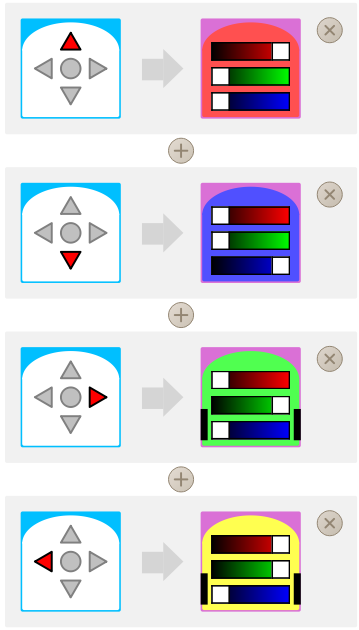
\includegraphics[width = 0.35\textwidth]{colors1}}
    \hspace{1cm}
    \subfigure[Éteindre Thymio lorsque le bouton centrale est pressé]{ \label{fig.colors-b} 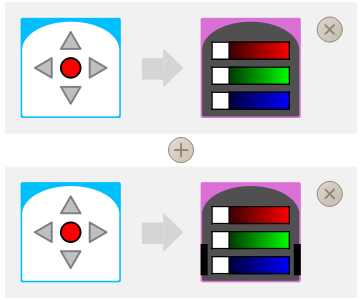
\includegraphics[width = 0.35\textwidth]{colors2}}
    \caption{Jouer avec les lumières de Thymio}
    \label{fig.colors}
\end{figure}

\begin{bclogo}[couleur = blue!30, arrondi = 0.1, logo = \bcinfo, ombre = true]{Trucs et astuces!}Lorsqu'un programme est lancé, toutes les paires d'événement-action sont actives.

Il est possible d'avoir plusieurs fois le même événement mais il \textbf{faut} que l'action correspondante soit différente! Si l'événement et l'action sont identiques, VPL vous indiquera qu'il y a une erreur.
\end{bclogo}




